\documentclass[11pt]{article}

% ============================================================================
% Structure and Obstructions in the Rule 30 Eventual-Periodicity Problem
% Comprehensive paper: proven results + period-2 census + obstruction register.
% Part I is lifted from zero-tail-note.tex (the standalone period-1 note).
% STATUS: in-progress draft. Section markers "% DRAFT:" flag expansion points.
% ============================================================================

\usepackage[T1]{fontenc}
\usepackage{amsmath,amssymb,amsthm}
\usepackage[margin=0.9in]{geometry}
\usepackage{microtype}
\usepackage{booktabs}
\usepackage{longtable}
\usepackage[hidelinks]{hyperref}
\hypersetup{
  pdftitle={Structure and Obstructions in the Rule 30 Eventual-Periodicity Problem},
  pdfauthor={David Lee Condrey}
}

% --- figures, lifted from zero-tail-note.tex along with Part I's proofs ---
\usepackage{tikz}
\usetikzlibrary{arrows.meta,positioning}
\usepackage{caption}
\captionsetup{font=small,labelfont=bf,skip=6pt}
\definecolor{ruleblue}{RGB}{31,78,121}
\definecolor{rulegold}{RGB}{191,125,17}
\definecolor{ruleink}{RGB}{23,33,48}
\definecolor{ruleband}{RGB}{250,232,199}
\tikzset{
  rulecard/.style={draw=ruleblue!70!black, line width=0.7pt,
    rounded corners=4pt, fill=ruleblue!4, inner sep=7pt, align=center,
    minimum height=1.38cm},
  rulecardfill/.style={fill=ruleblue!4, rounded corners=2.4pt},
  rulecardline/.style={draw=ruleblue!70!black, line width=0.6pt,
    rounded corners=2.4pt},
  rulearrow/.style={-{Latex[length=2.8mm]}, very thick, rulegold!90!black},
}
\newcommand{\stlabel}[1]{{\small\textcolor{ruleblue!90!black}{\bfseries #1}}}
\newcommand{\stnote}[1]{{\small\textcolor{rulegold!90!black}{\bfseries #1}}}
\newcommand{\stpanel}[3]{%
  \begin{tabular}[t]{@{}c@{}}
    \stlabel{#1}\\[0.5pt]
    {\scriptsize #2}\\[3.5pt]
    #3
  \end{tabular}}

\newtheorem{theorem}{Theorem}[section]
\newtheorem{lemma}[theorem]{Lemma}
\newtheorem{corollary}[theorem]{Corollary}
\newtheorem{proposition}[theorem]{Proposition}
\theoremstyle{definition}
\newtheorem{conjecture}[theorem]{Conjecture}
\newtheorem{observation}[theorem]{Observation}
\newtheorem{remark}[theorem]{Remark}

\newcommand{\F}{\mathcal F}
\newcommand{\Tr}{\operatorname{Tr}}
\newcommand{\supp}{\operatorname{supp}}
\newcommand{\gm}{\gamma}

\title{\vspace{-2em}Structure and Obstructions in the\\Rule 30 Eventual-Periodicity Problem}
\author{David Lee Condrey\\WritersLogic, Inc.\\\texttt{david@writerslogic.com}}
\date{September 2026}

\begin{document}
\maketitle

\begin{abstract}
Wolfram's Prize Problem~1 asks whether the center column of the lone-seed
Rule~30 orbit always remains non-periodic. We do not resolve it, and we say so
at the outset: Problems~1, 2 and 3 remain open. What we contribute is a structured
account of the boundary between what is provable and what is not for this
problem. First, we settle the entire eventual-period-\emph{one} subcase for
every nonzero finite configuration, a class strictly broader than the lone
seed: the two constant-trace fibers are computed exactly, neither meets the
finitely supported configurations away from the origin, and the sharp
constant-prefix horizon is $w+2$ for support radius $w$. Second, we delimit the
eventual-period-\emph{two} case from two sides: a mechanized
$\omega$-automaton periodicity ladder, for which we prove three separate
limitation theorems (its verdict is uniform in right depth, in left depth, and
in the diagonal bound, so none of its levers can close the case); and an
exhaustive forced-continuation census, which we carry to source length $n=24$
exhaustively and $n=30$ by a verified fast method, finding that the exclusion is
decided not by a thinning population but by a bounded handful of extremal
forcing states. Third, and this is the paper's methodological purpose, we give
the first structured register of the attacks that fail on this problem:
ninety-four distinct routes, organized into nine obstruction classes, each with
its exact kill reason, and all unified by a single fact --- Rule~30's
\textsc{or} nonlinearity is the only property separating it from the additive
Rule~90, whose center column \emph{is} eventually periodic, so any argument that
does not use that nonlinearity cannot succeed. The register is the map the field
currently lacks. An exhaustive per-route compendium and the full computational
archive accompany the paper as a supplement and a data deposit.
\end{abstract}

\tableofcontents

% ============================================================================
\section{Introduction}
% ============================================================================

Rule~30 is the binary cellular automaton on $\{0,1\}^{\mathbb Z}$ with local rule
\begin{equation}\label{eq:rule30}
 F(x)_i=x_{i-1}\oplus(x_i\lor x_{i+1}),
\end{equation}
left permutive: fixing $x_i,x_{i+1}$, the value $F(x)_i$ is a bijection of
$x_{i-1}$.

Wolfram poses three problems about the center column of the lone-seed orbit and
offers \$10{,}000 for each \cite{wolfram}. Problem~1 asks ``Does the center
column always remain non-periodic?''; Problem~2, ``Does each color of cell occur
on average equally often in the center column?''; and Problem~3, ``Does
computing the $n$th cell of the center column require at least $O(n)$
computational effort?'' A solution is a proof over the traditional axioms of
standard mathematics. The column is verified non-periodic only through the first
$10^9$ steps; as Wolfram notes, ``there could be a trillion-step transient,
after which it's periodic,'' so no finite check can settle Problem~1 --- a limit
we return to as obstruction~H (Section~\ref{sec:register}). We address Problem~1
throughout, Problem~2 through the period-two thread, and Problem~3 only in the
register.

Kopra records the broader finite-configuration version of Problem~1 as open
\cite{kopra-thesis}. Jen proved a finite orbit has at most one eventually
periodic column \cite[Thm.~2b]{jen1986}\cite[Prop.~3]{jen}; Kopra proved the
width-two column is never eventually periodic but left width one open, and
showed his technique cannot reach it \cite{kopra}.

This paper is organized around one fact that we make load-bearing throughout.
Rule~90, $F(x)_i = x_{i-1}\oplus x_{i+1}$, is also left permutive, yet its
lone-seed center column \emph{is} eventually periodic (identically zero off the
initial step). Hence no argument that uses only left permutivity, additivity, or
any property Rule~90 shares can decide Problem~1: it would prove a false
statement about Rule~90. The single property Rule~30 has that Rule~90 lacks is
the \textsc{or} in \eqref{eq:rule30}, which latches. We call the requirement that
an argument depend on this latch the \emph{Rule~90 filter}. Every positive
result below passes it; every failure catalogued in Part~IV either violates it
or hits one of eight further walls.

\paragraph{What is proved.} Part~I settles eventual period one
(Section~\ref{sec:periodone}): both constant-trace fibers are computed in closed
form, the finite configurations meet them only at the origin, and the horizon is
sharp. Part~III proves three limitation theorems for the period-two ladder
(Section~\ref{sec:ladder}). These are honest negative results: they say a
specific, natural, mechanized method cannot close period two, and why.

\paragraph{What is measured, and what is conjectured.} Part~II
(Section~\ref{sec:periodtwo}) reduces period-two exclusion to a finite-word
statement, carries the exhaustive census to $n=24$ (and a verified fast method to
$n=30$), and reports a structural phenomenon: near extinction the surviving
witnesses collapse onto $O(1)$ extremal forcing states sharing a long common
suffix and a single failure symbol. We state this as a conjecture with its
supporting data, never as a theorem.

\paragraph{What fails, and why.} Part~IV (Section~\ref{sec:register}) is the
register. Nine obstruction classes account for the ninety-four
routes attempted across this project. We give each class, the routes it kills,
the kill-reason type, and its Rule~90 status. The exhaustive per-route list is
the accompanying supplement.

\paragraph{Scope.} Part~V (Section~\ref{sec:scope}) states precisely what is and
is not reached, against the published state of the art, and lists the concrete
open leads. We claim no progress on the prize problems themselves.

% ============================================================================
\section{Part I: Finite configurations cannot generate a constant trace}
\label{sec:periodone}
% ============================================================================

This part is lifted, statement and proof, from the standalone note
\texttt{zero-tail-note.tex}, which carries the full hostile-audited derivation,
the Lean and SMT certificates, and the reproducibility appendix; only the two
figures and the eight results are reproduced here.

We write $c_t:=\Tr(x)_t=F^t(x)_0$, $R_j:=x_j$, $L_j:=x_{-j}$ ($j\ge0$), and let
$\F$ denote the finitely supported configurations. The trace sees only column
$0$, but under a left-permutive rule a discrepancy left of the origin
propagates rightward along a diagonal and must eventually reach it. The
classification rests on this one fact, which uses only locality and left
permutivity, not the specific form of \eqref{eq:rule30}.

\begin{lemma}[Triangular uniqueness]\label{lem:unique}
If two configurations agree at every coordinate $i\ge0$ and have the same
central trace, then they are equal.
\end{lemma}
\begin{proof}
If $-n$ is their rightmost differing coordinate, locality preserves agreement
to its right through time $n$. Left permutivity preserves the discrepancy
along $(-n,0),(-n+1,1),\dots,(0,n)$, contradicting equal traces. In its finite
form, if the rows agree on $i\ge0$ and their traces agree for $0\le t\le r$,
the same induction forces agreement at $-r,-r+1,\dots,-1$.
\end{proof}

Uniqueness alone does not say what the forced left half looks like. The next
result computes it: the rows with zero trace form one invariant class
$\mathcal C_m$ for each position $m$ of the first right-hand one, each class is
carried to its predecessor by $F$, and the left half is a prefix-OR of the
right. Figure~\ref{fig:panels}(a) is a member of $\mathcal C_3$.

\begin{theorem}[Zero-trace fiber]\label{thm:fiber}
For a prescribed right half with $R_0=0$, the zero-trace-compatible left half is
unique. If the positive half is nonzero and $m=\min\{j\ge1:R_j=1\}$, the forced
left half is $L_j=0\ (j<m)$, $L_m=1$, $L_j=j\bmod2\ (j>m)$, with $R_j$ for
$j>m$ arbitrary. If instead the positive half is zero, the unique row is zero.
Equivalently, in prefix-OR form,
\begin{align}
 L_{2k+1}&=\bigvee_{j=1}^{2k+1}R_j &&(k\ge0),\\[-2pt]
 L_{2k}&=R_{2k}\land\neg\!\bigvee_{j=1}^{2k-1}R_j &&(k\ge1).
\end{align}
\end{theorem}
\begin{proof}
For $m\ge1$, let $\mathcal C_m$ consist of rows satisfying these conditions.
One Rule~30 step gives
\begin{equation}\label{eq:updates}
\begin{aligned}
 x'_0&=L_1\oplus R_1, &
 R'_j&=R_{j-1}\oplus(R_j\lor R_{j+1}), &
 L'_j&=L_{j+1}\oplus(L_j\lor L_{j-1}).
\end{aligned}
\end{equation}
Suppose $m>1$. These identities give $x'_0=0$, $R'_j=L'_j=0\ (j<m-1)$,
$R'_{m-1}=L'_{m-1}=1$, $L'_m=m\bmod2$. For $j>m$, including $j=m+1$ because
$L_m=1$, the OR in the last update is one, so $L'_j=(1-(j\bmod2))\oplus1=j\bmod2$.
Thus $F(\mathcal C_m)\subseteq\mathcal C_{m-1}$. For $m=1$, the alternating left
half is fixed, $x'_0=1\oplus1=0$, and $R'_1=0\oplus(1\lor R_2)=1$ independently
of the right tail; hence $F(\mathcal C_1)\subseteq\mathcal C_1$. Every
$\mathcal C_m$ therefore realizes the zero trace. A nonzero right half selects a
realization by its first one, and Lemma~\ref{lem:unique} makes it unique; a
zero right half forces a zero left half by the same lemma against the zero row.
\end{proof}

\begin{figure}[t]
\centering
\begin{tabular}{@{}c@{\hspace{7mm}}c@{\hspace{7mm}}c@{}}
\stpanel{(a) Rule 30}{class $\mathcal C_3$, center zero}{%
  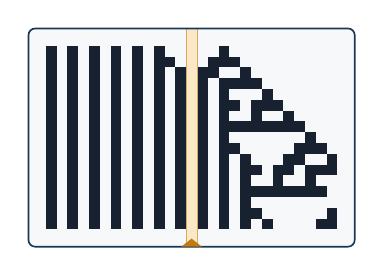
\begin{tikzpicture}[scale=2.365]  \fill[rulecardfill] (-0.8468,0.0928) rectangle (0.9048,-1.0788);
  \fill[ruleband] (0.0000,0.0928) rectangle (0.0580,-1.0788);
  \fill[ruleink] (0.1740,0.0000) rectangle ++(0.0580,-0.0580);
  \fill[ruleink] (-0.7540,0.0000) rectangle ++(0.0580,-0.0580);
  \fill[ruleink] (-0.6380,0.0000) rectangle ++(0.0580,-0.0580);
  \fill[ruleink] (-0.5220,0.0000) rectangle ++(0.0580,-0.0580);
  \fill[ruleink] (-0.4060,0.0000) rectangle ++(0.0580,-0.0580);
  \fill[ruleink] (-0.2900,0.0000) rectangle ++(0.0580,-0.0580);
  \fill[ruleink] (-0.1740,0.0000) rectangle ++(0.0580,-0.0580);
  \fill[ruleink] (0.1160,-0.0580) rectangle ++(0.0580,-0.0580);
  \fill[ruleink] (0.1740,-0.0580) rectangle ++(0.0580,-0.0580);
  \fill[ruleink] (0.2320,-0.0580) rectangle ++(0.0580,-0.0580);
  \fill[ruleink] (-0.7540,-0.0580) rectangle ++(0.0580,-0.0580);
  \fill[ruleink] (-0.6380,-0.0580) rectangle ++(0.0580,-0.0580);
  \fill[ruleink] (-0.5220,-0.0580) rectangle ++(0.0580,-0.0580);
  \fill[ruleink] (-0.4060,-0.0580) rectangle ++(0.0580,-0.0580);
  \fill[ruleink] (-0.2900,-0.0580) rectangle ++(0.0580,-0.0580);
  \fill[ruleink] (-0.1740,-0.0580) rectangle ++(0.0580,-0.0580);
  \fill[ruleink] (-0.1160,-0.0580) rectangle ++(0.0580,-0.0580);
  \fill[ruleink] (0.0580,-0.1160) rectangle ++(0.0580,-0.0580);
  \fill[ruleink] (0.1160,-0.1160) rectangle ++(0.0580,-0.0580);
  \fill[ruleink] (0.2900,-0.1160) rectangle ++(0.0580,-0.0580);
  \fill[ruleink] (-0.7540,-0.1160) rectangle ++(0.0580,-0.0580);
  \fill[ruleink] (-0.6380,-0.1160) rectangle ++(0.0580,-0.0580);
  \fill[ruleink] (-0.5220,-0.1160) rectangle ++(0.0580,-0.0580);
  \fill[ruleink] (-0.4060,-0.1160) rectangle ++(0.0580,-0.0580);
  \fill[ruleink] (-0.2900,-0.1160) rectangle ++(0.0580,-0.0580);
  \fill[ruleink] (-0.1740,-0.1160) rectangle ++(0.0580,-0.0580);
  \fill[ruleink] (-0.0580,-0.1160) rectangle ++(0.0580,-0.0580);
  \fill[ruleink] (0.0580,-0.1740) rectangle ++(0.0580,-0.0580);
  \fill[ruleink] (0.1740,-0.1740) rectangle ++(0.0580,-0.0580);
  \fill[ruleink] (0.2320,-0.1740) rectangle ++(0.0580,-0.0580);
  \fill[ruleink] (0.2900,-0.1740) rectangle ++(0.0580,-0.0580);
  \fill[ruleink] (0.3480,-0.1740) rectangle ++(0.0580,-0.0580);
  \fill[ruleink] (-0.7540,-0.1740) rectangle ++(0.0580,-0.0580);
  \fill[ruleink] (-0.6380,-0.1740) rectangle ++(0.0580,-0.0580);
  \fill[ruleink] (-0.5220,-0.1740) rectangle ++(0.0580,-0.0580);
  \fill[ruleink] (-0.4060,-0.1740) rectangle ++(0.0580,-0.0580);
  \fill[ruleink] (-0.2900,-0.1740) rectangle ++(0.0580,-0.0580);
  \fill[ruleink] (-0.1740,-0.1740) rectangle ++(0.0580,-0.0580);
  \fill[ruleink] (-0.0580,-0.1740) rectangle ++(0.0580,-0.0580);
  \fill[ruleink] (0.0580,-0.2320) rectangle ++(0.0580,-0.0580);
  \fill[ruleink] (0.1740,-0.2320) rectangle ++(0.0580,-0.0580);
  \fill[ruleink] (0.4060,-0.2320) rectangle ++(0.0580,-0.0580);
  \fill[ruleink] (-0.7540,-0.2320) rectangle ++(0.0580,-0.0580);
  \fill[ruleink] (-0.6380,-0.2320) rectangle ++(0.0580,-0.0580);
  \fill[ruleink] (-0.5220,-0.2320) rectangle ++(0.0580,-0.0580);
  \fill[ruleink] (-0.4060,-0.2320) rectangle ++(0.0580,-0.0580);
  \fill[ruleink] (-0.2900,-0.2320) rectangle ++(0.0580,-0.0580);
  \fill[ruleink] (-0.1740,-0.2320) rectangle ++(0.0580,-0.0580);
  \fill[ruleink] (-0.0580,-0.2320) rectangle ++(0.0580,-0.0580);
  \fill[ruleink] (0.0580,-0.2900) rectangle ++(0.0580,-0.0580);
  \fill[ruleink] (0.1740,-0.2900) rectangle ++(0.0580,-0.0580);
  \fill[ruleink] (0.2320,-0.2900) rectangle ++(0.0580,-0.0580);
  \fill[ruleink] (0.3480,-0.2900) rectangle ++(0.0580,-0.0580);
  \fill[ruleink] (0.4060,-0.2900) rectangle ++(0.0580,-0.0580);
  \fill[ruleink] (0.4640,-0.2900) rectangle ++(0.0580,-0.0580);
  \fill[ruleink] (-0.7540,-0.2900) rectangle ++(0.0580,-0.0580);
  \fill[ruleink] (-0.6380,-0.2900) rectangle ++(0.0580,-0.0580);
  \fill[ruleink] (-0.5220,-0.2900) rectangle ++(0.0580,-0.0580);
  \fill[ruleink] (-0.4060,-0.2900) rectangle ++(0.0580,-0.0580);
  \fill[ruleink] (-0.2900,-0.2900) rectangle ++(0.0580,-0.0580);
  \fill[ruleink] (-0.1740,-0.2900) rectangle ++(0.0580,-0.0580);
  \fill[ruleink] (-0.0580,-0.2900) rectangle ++(0.0580,-0.0580);
  \fill[ruleink] (0.0580,-0.3480) rectangle ++(0.0580,-0.0580);
  \fill[ruleink] (0.1740,-0.3480) rectangle ++(0.0580,-0.0580);
  \fill[ruleink] (0.3480,-0.3480) rectangle ++(0.0580,-0.0580);
  \fill[ruleink] (0.5220,-0.3480) rectangle ++(0.0580,-0.0580);
  \fill[ruleink] (-0.7540,-0.3480) rectangle ++(0.0580,-0.0580);
  \fill[ruleink] (-0.6380,-0.3480) rectangle ++(0.0580,-0.0580);
  \fill[ruleink] (-0.5220,-0.3480) rectangle ++(0.0580,-0.0580);
  \fill[ruleink] (-0.4060,-0.3480) rectangle ++(0.0580,-0.0580);
  \fill[ruleink] (-0.2900,-0.3480) rectangle ++(0.0580,-0.0580);
  \fill[ruleink] (-0.1740,-0.3480) rectangle ++(0.0580,-0.0580);
  \fill[ruleink] (-0.0580,-0.3480) rectangle ++(0.0580,-0.0580);
  \fill[ruleink] (0.0580,-0.4060) rectangle ++(0.0580,-0.0580);
  \fill[ruleink] (0.1740,-0.4060) rectangle ++(0.0580,-0.0580);
  \fill[ruleink] (0.2320,-0.4060) rectangle ++(0.0580,-0.0580);
  \fill[ruleink] (0.2900,-0.4060) rectangle ++(0.0580,-0.0580);
  \fill[ruleink] (0.3480,-0.4060) rectangle ++(0.0580,-0.0580);
  \fill[ruleink] (0.4060,-0.4060) rectangle ++(0.0580,-0.0580);
  \fill[ruleink] (0.4640,-0.4060) rectangle ++(0.0580,-0.0580);
  \fill[ruleink] (0.5220,-0.4060) rectangle ++(0.0580,-0.0580);
  \fill[ruleink] (0.5800,-0.4060) rectangle ++(0.0580,-0.0580);
  \fill[ruleink] (-0.7540,-0.4060) rectangle ++(0.0580,-0.0580);
  \fill[ruleink] (-0.6380,-0.4060) rectangle ++(0.0580,-0.0580);
  \fill[ruleink] (-0.5220,-0.4060) rectangle ++(0.0580,-0.0580);
  \fill[ruleink] (-0.4060,-0.4060) rectangle ++(0.0580,-0.0580);
  \fill[ruleink] (-0.2900,-0.4060) rectangle ++(0.0580,-0.0580);
  \fill[ruleink] (-0.1740,-0.4060) rectangle ++(0.0580,-0.0580);
  \fill[ruleink] (-0.0580,-0.4060) rectangle ++(0.0580,-0.0580);
  \fill[ruleink] (0.0580,-0.4640) rectangle ++(0.0580,-0.0580);
  \fill[ruleink] (0.1740,-0.4640) rectangle ++(0.0580,-0.0580);
  \fill[ruleink] (0.6380,-0.4640) rectangle ++(0.0580,-0.0580);
  \fill[ruleink] (-0.7540,-0.4640) rectangle ++(0.0580,-0.0580);
  \fill[ruleink] (-0.6380,-0.4640) rectangle ++(0.0580,-0.0580);
  \fill[ruleink] (-0.5220,-0.4640) rectangle ++(0.0580,-0.0580);
  \fill[ruleink] (-0.4060,-0.4640) rectangle ++(0.0580,-0.0580);
  \fill[ruleink] (-0.2900,-0.4640) rectangle ++(0.0580,-0.0580);
  \fill[ruleink] (-0.1740,-0.4640) rectangle ++(0.0580,-0.0580);
  \fill[ruleink] (-0.0580,-0.4640) rectangle ++(0.0580,-0.0580);
  \fill[ruleink] (0.0580,-0.5220) rectangle ++(0.0580,-0.0580);
  \fill[ruleink] (0.1740,-0.5220) rectangle ++(0.0580,-0.0580);
  \fill[ruleink] (0.2320,-0.5220) rectangle ++(0.0580,-0.0580);
  \fill[ruleink] (0.5800,-0.5220) rectangle ++(0.0580,-0.0580);
  \fill[ruleink] (0.6380,-0.5220) rectangle ++(0.0580,-0.0580);
  \fill[ruleink] (0.6960,-0.5220) rectangle ++(0.0580,-0.0580);
  \fill[ruleink] (-0.7540,-0.5220) rectangle ++(0.0580,-0.0580);
  \fill[ruleink] (-0.6380,-0.5220) rectangle ++(0.0580,-0.0580);
  \fill[ruleink] (-0.5220,-0.5220) rectangle ++(0.0580,-0.0580);
  \fill[ruleink] (-0.4060,-0.5220) rectangle ++(0.0580,-0.0580);
  \fill[ruleink] (-0.2900,-0.5220) rectangle ++(0.0580,-0.0580);
  \fill[ruleink] (-0.1740,-0.5220) rectangle ++(0.0580,-0.0580);
  \fill[ruleink] (-0.0580,-0.5220) rectangle ++(0.0580,-0.0580);
  \fill[ruleink] (0.0580,-0.5800) rectangle ++(0.0580,-0.0580);
  \fill[ruleink] (0.1740,-0.5800) rectangle ++(0.0580,-0.0580);
  \fill[ruleink] (0.2900,-0.5800) rectangle ++(0.0580,-0.0580);
  \fill[ruleink] (0.5220,-0.5800) rectangle ++(0.0580,-0.0580);
  \fill[ruleink] (0.5800,-0.5800) rectangle ++(0.0580,-0.0580);
  \fill[ruleink] (0.7540,-0.5800) rectangle ++(0.0580,-0.0580);
  \fill[ruleink] (-0.7540,-0.5800) rectangle ++(0.0580,-0.0580);
  \fill[ruleink] (-0.6380,-0.5800) rectangle ++(0.0580,-0.0580);
  \fill[ruleink] (-0.5220,-0.5800) rectangle ++(0.0580,-0.0580);
  \fill[ruleink] (-0.4060,-0.5800) rectangle ++(0.0580,-0.0580);
  \fill[ruleink] (-0.2900,-0.5800) rectangle ++(0.0580,-0.0580);
  \fill[ruleink] (-0.1740,-0.5800) rectangle ++(0.0580,-0.0580);
  \fill[ruleink] (-0.0580,-0.5800) rectangle ++(0.0580,-0.0580);
  \fill[ruleink] (0.0580,-0.6380) rectangle ++(0.0580,-0.0580);
  \fill[ruleink] (0.1740,-0.6380) rectangle ++(0.0580,-0.0580);
  \fill[ruleink] (0.2900,-0.6380) rectangle ++(0.0580,-0.0580);
  \fill[ruleink] (0.3480,-0.6380) rectangle ++(0.0580,-0.0580);
  \fill[ruleink] (0.4640,-0.6380) rectangle ++(0.0580,-0.0580);
  \fill[ruleink] (0.5220,-0.6380) rectangle ++(0.0580,-0.0580);
  \fill[ruleink] (0.6380,-0.6380) rectangle ++(0.0580,-0.0580);
  \fill[ruleink] (0.6960,-0.6380) rectangle ++(0.0580,-0.0580);
  \fill[ruleink] (0.7540,-0.6380) rectangle ++(0.0580,-0.0580);
  \fill[ruleink] (-0.7540,-0.6380) rectangle ++(0.0580,-0.0580);
  \fill[ruleink] (-0.6380,-0.6380) rectangle ++(0.0580,-0.0580);
  \fill[ruleink] (-0.5220,-0.6380) rectangle ++(0.0580,-0.0580);
  \fill[ruleink] (-0.4060,-0.6380) rectangle ++(0.0580,-0.0580);
  \fill[ruleink] (-0.2900,-0.6380) rectangle ++(0.0580,-0.0580);
  \fill[ruleink] (-0.1740,-0.6380) rectangle ++(0.0580,-0.0580);
  \fill[ruleink] (-0.0580,-0.6380) rectangle ++(0.0580,-0.0580);
  \fill[ruleink] (0.0580,-0.6960) rectangle ++(0.0580,-0.0580);
  \fill[ruleink] (0.1740,-0.6960) rectangle ++(0.0580,-0.0580);
  \fill[ruleink] (0.2900,-0.6960) rectangle ++(0.0580,-0.0580);
  \fill[ruleink] (0.4640,-0.6960) rectangle ++(0.0580,-0.0580);
  \fill[ruleink] (0.6380,-0.6960) rectangle ++(0.0580,-0.0580);
  \fill[ruleink] (-0.7540,-0.6960) rectangle ++(0.0580,-0.0580);
  \fill[ruleink] (-0.6380,-0.6960) rectangle ++(0.0580,-0.0580);
  \fill[ruleink] (-0.5220,-0.6960) rectangle ++(0.0580,-0.0580);
  \fill[ruleink] (-0.4060,-0.6960) rectangle ++(0.0580,-0.0580);
  \fill[ruleink] (-0.2900,-0.6960) rectangle ++(0.0580,-0.0580);
  \fill[ruleink] (-0.1740,-0.6960) rectangle ++(0.0580,-0.0580);
  \fill[ruleink] (-0.0580,-0.6960) rectangle ++(0.0580,-0.0580);
  \fill[ruleink] (0.0580,-0.7540) rectangle ++(0.0580,-0.0580);
  \fill[ruleink] (0.1740,-0.7540) rectangle ++(0.0580,-0.0580);
  \fill[ruleink] (0.2900,-0.7540) rectangle ++(0.0580,-0.0580);
  \fill[ruleink] (0.3480,-0.7540) rectangle ++(0.0580,-0.0580);
  \fill[ruleink] (0.4060,-0.7540) rectangle ++(0.0580,-0.0580);
  \fill[ruleink] (0.4640,-0.7540) rectangle ++(0.0580,-0.0580);
  \fill[ruleink] (0.5220,-0.7540) rectangle ++(0.0580,-0.0580);
  \fill[ruleink] (0.5800,-0.7540) rectangle ++(0.0580,-0.0580);
  \fill[ruleink] (0.6380,-0.7540) rectangle ++(0.0580,-0.0580);
  \fill[ruleink] (0.6960,-0.7540) rectangle ++(0.0580,-0.0580);
  \fill[ruleink] (-0.7540,-0.7540) rectangle ++(0.0580,-0.0580);
  \fill[ruleink] (-0.6380,-0.7540) rectangle ++(0.0580,-0.0580);
  \fill[ruleink] (-0.5220,-0.7540) rectangle ++(0.0580,-0.0580);
  \fill[ruleink] (-0.4060,-0.7540) rectangle ++(0.0580,-0.0580);
  \fill[ruleink] (-0.2900,-0.7540) rectangle ++(0.0580,-0.0580);
  \fill[ruleink] (-0.1740,-0.7540) rectangle ++(0.0580,-0.0580);
  \fill[ruleink] (-0.0580,-0.7540) rectangle ++(0.0580,-0.0580);
  \fill[ruleink] (0.0580,-0.8120) rectangle ++(0.0580,-0.0580);
  \fill[ruleink] (0.1740,-0.8120) rectangle ++(0.0580,-0.0580);
  \fill[ruleink] (0.2900,-0.8120) rectangle ++(0.0580,-0.0580);
  \fill[ruleink] (-0.7540,-0.8120) rectangle ++(0.0580,-0.0580);
  \fill[ruleink] (-0.6380,-0.8120) rectangle ++(0.0580,-0.0580);
  \fill[ruleink] (-0.5220,-0.8120) rectangle ++(0.0580,-0.0580);
  \fill[ruleink] (-0.4060,-0.8120) rectangle ++(0.0580,-0.0580);
  \fill[ruleink] (-0.2900,-0.8120) rectangle ++(0.0580,-0.0580);
  \fill[ruleink] (-0.1740,-0.8120) rectangle ++(0.0580,-0.0580);
  \fill[ruleink] (-0.0580,-0.8120) rectangle ++(0.0580,-0.0580);
  \fill[ruleink] (0.0580,-0.8700) rectangle ++(0.0580,-0.0580);
  \fill[ruleink] (0.1740,-0.8700) rectangle ++(0.0580,-0.0580);
  \fill[ruleink] (0.2900,-0.8700) rectangle ++(0.0580,-0.0580);
  \fill[ruleink] (0.3480,-0.8700) rectangle ++(0.0580,-0.0580);
  \fill[ruleink] (0.7540,-0.8700) rectangle ++(0.0580,-0.0580);
  \fill[ruleink] (-0.7540,-0.8700) rectangle ++(0.0580,-0.0580);
  \fill[ruleink] (-0.6380,-0.8700) rectangle ++(0.0580,-0.0580);
  \fill[ruleink] (-0.5220,-0.8700) rectangle ++(0.0580,-0.0580);
  \fill[ruleink] (-0.4060,-0.8700) rectangle ++(0.0580,-0.0580);
  \fill[ruleink] (-0.2900,-0.8700) rectangle ++(0.0580,-0.0580);
  \fill[ruleink] (-0.1740,-0.8700) rectangle ++(0.0580,-0.0580);
  \fill[ruleink] (-0.0580,-0.8700) rectangle ++(0.0580,-0.0580);
  \fill[ruleink] (0.0580,-0.9280) rectangle ++(0.0580,-0.0580);
  \fill[ruleink] (0.1740,-0.9280) rectangle ++(0.0580,-0.0580);
  \fill[ruleink] (0.2900,-0.9280) rectangle ++(0.0580,-0.0580);
  \fill[ruleink] (0.4060,-0.9280) rectangle ++(0.0580,-0.0580);
  \fill[ruleink] (0.6960,-0.9280) rectangle ++(0.0580,-0.0580);
  \fill[ruleink] (0.7540,-0.9280) rectangle ++(0.0580,-0.0580);
  \fill[ruleink] (-0.7540,-0.9280) rectangle ++(0.0580,-0.0580);
  \fill[ruleink] (-0.6380,-0.9280) rectangle ++(0.0580,-0.0580);
  \fill[ruleink] (-0.5220,-0.9280) rectangle ++(0.0580,-0.0580);
  \fill[ruleink] (-0.4060,-0.9280) rectangle ++(0.0580,-0.0580);
  \fill[ruleink] (-0.2900,-0.9280) rectangle ++(0.0580,-0.0580);
  \fill[ruleink] (-0.1740,-0.9280) rectangle ++(0.0580,-0.0580);
  \fill[ruleink] (-0.0580,-0.9280) rectangle ++(0.0580,-0.0580);
  \draw[rulegold!65, line width=0.3pt] (0.0000,0.0928) -- (0.0000,-1.0788);
  \draw[rulegold!65, line width=0.3pt] (0.0580,0.0928) -- (0.0580,-1.0788);
  \draw[rulecardline] (-0.8468,0.0928) rectangle (0.9048,-1.0788);
  \fill[rulegold] (-0.0261,-1.0788) -- (0.0841,-1.0788) -- (0.0290,-1.0353) -- cycle;
\end{tikzpicture}}
&
\stpanel{(b) Rule 90}{$x=\delta_{-1}+\delta_{1}$, center zero}{%
  \begin{tikzpicture}[scale=2.365]\input{figures/fig-rule90}\end{tikzpicture}}
&
\stpanel{(c) Rule 30}{same row, center escapes}{%
  \begin{tikzpicture}[scale=2.365]\input{figures/fig-rule30}\end{tikzpicture}}
\end{tabular}
\\[3mm]
\stnote{gold band and caret mark column $0$}
\caption{Time runs downward. In (a) the forced left tail alternates, hence is
infinite, which is what Corollary~\ref{cor:finite} exploits. Panels (b) and
(c) run one finite row under both rules; the difference is the OR latch in
\eqref{eq:rule30}.}
\label{fig:panels}
\end{figure}

The other constant trace has a simpler fiber: one row per right half, and the
left half no longer depends on which right half it is.

\begin{theorem}[All-one fiber]\label{thm:onefiber}
For a prescribed right half with $R_0=1$, the left half compatible with an
identically-one trace is unique and independent of the right half:
$L_j=1\iff j$ is positive and even.
\end{theorem}
\begin{proof}
Write $L_0:=x_0=R_0=1$, so the third identity of \eqref{eq:updates},
$L'_j=L_{j+1}\oplus(L_j\lor L_{j-1})$, applies at every $j\ge1$. Under the
checkerboard pattern it gives $0\oplus(1\lor0)=1$ for even $j$ and
$1\oplus(0\lor1)=0$ for odd $j$, so the left half is fixed by $F$ whatever the
right half is. At the origin, $F(x)_0=L_1\oplus(L_0\lor R_1)=0\oplus1=1$
independently of $R_1$, so the trace is identically one and $L_0=1$ is restored
at every step. Lemma~\ref{lem:unique} makes the left half unique.
\end{proof}

Every nonzero row in Theorem~\ref{thm:fiber} carries ones arbitrarily far to
the left, so none of them is finitely supported. That is the whole of the next
statement, once one checks that a finite orbit cannot become the zero row.

\begin{corollary}\label{cor:finite}
$\Tr^{-1}(0^{\mathbb N})\cap\F=\{0\}$. Moreover, no column of the orbit of a
nonzero $x\in\F$ is eventually zero.
\end{corollary}
\begin{proof}
Every nonzero row in Theorem~\ref{thm:fiber} has ones at all sufficiently large
odd left depths. If a column of a finite orbit were zero from time $T$ onward,
translation would make $F^T(x)$ a finite zero-trace row. It is nonzero: if
$[a,b]$ is the support interval of a nonzero finite row, its next row has ones
at $a-1$ and $b+1$ because Rule~30 maps $001$ and $100$ to one.
\end{proof}

Corollary~\ref{cor:finite} is not a consequence of left permutivity alone:
Rule~90 is also left permutive, yet the finite row with ones at $\pm1$ keeps a
zero center forever (Figure~\ref{fig:panels}(b,c)). The Rule-30-specific step
is the OR latch $R'_1=1\lor R_2=1$ in the proof of Theorem~\ref{thm:fiber},
which has no analogue in an additive rule.

The same latch upgrades the corollary from one constant to both, with no
further machinery. Theorem~\ref{thm:onefiber} proves the second half again and
independently, since the checkerboard pattern has ones at every positive even
depth; the argument below is shorter and is the one to quote.

\begin{corollary}\label{cor:constant}
No column of the orbit of a nonzero $x\in\F$ is eventually constant.
\end{corollary}
\begin{proof}
The eventually-zero case is Corollary~\ref{cor:finite}. Suppose instead some
column is eventually one; translating, take it to be column $0$, so $c_t=1$
for all $t\ge T$. Applying \eqref{eq:rule30} at the origin gives
$l_t=c_{t+1}\oplus(c_t\lor r_t)$, and $c_t=1$ collapses the disjunction, so
$l_t=1\oplus c_{t+1}$. For $t\ge T$ we also have $c_{t+1}=1$, hence $l_t=0$.
Column $-1$ is then zero from time $T$ onward, which Corollary~\ref{cor:finite}
forbids.
\end{proof}

Corollary~\ref{cor:finite} says a finite row's center cannot stay zero forever.
How long it can stay zero, as a function of the support radius, is exactly one
step past the light cone of the first odd depth beyond that radius. For $w\ge1$
let $\mathcal S_w=\{x\ne0:\supp(x)\subseteq[-w,w],x_0=0\}$, and for
$x\in\mathcal S_w$ let $H(x)=\max\{h:F^t(x)_0=0\text{ for }0\le t\le h\}$.

\begin{theorem}[Sharp finite horizon]\label{thm:horizon}
Let $w\ge1$. Then
\begin{equation}
 \max_{x\in\mathcal S_w}H(x)=2\left\lceil\frac w2\right\rceil,\qquad
 \#\!\left\{x\in\mathcal S_w:H(x)=2\left\lceil\frac w2\right\rceil\right\}=2^w-1.
\end{equation}
\end{theorem}
\begin{proof}
Let $q$ be the least odd integer greater than $w$, so $q-1=2\lceil w/2\rceil$.
If the positive right half is nonzero, a trace zero through time $q$, compared
with its zero-trace completion, would force by finite-prefix uniqueness and
the prefix-OR identity $x_{-q}=\bigvee_{j=1}^qR_j=1$, contradicting $q>w$. If
that half is zero, comparison with the zero row makes every nonzero left cell
visible by time $w$. Thus $H(x)\le q-1$. Conversely, choose any of the $2^w-1$
nonzero words $(R_1,\dots,R_w)$, install the prefix-OR pattern through left
depth $w$, and zero all other cells. This row agrees with its infinite
zero-trace completion through the light cone of time $q-1$; when $w$ is odd,
the extra depth $w+1$ is even and forced to zero. The missing odd cell at depth
$q$ creates a discrepancy at time $q$, and finite-prefix uniqueness excludes
further extremizers.
\end{proof}

\begin{figure}[t]
\centering
\begin{tabular}{@{}c@{\hspace{5mm}}c@{\hspace{5mm}}c@{}}
\stlabel{$w=1$} & \stlabel{$w=2$} & \stlabel{$w=3$}
\\[3pt]

\begin{tikzpicture}[scale=2.8224]  \fill[rulecardfill] (-0.3828,0.0928) rectangle (0.4408,-0.3248);
  \fill[ruleband] (0.0000,0.0928) rectangle (0.0580,-0.3248);
  \fill[ruleink] (0.0580,0.0000) rectangle ++(0.0580,-0.0580);
  \fill[ruleink] (-0.0580,0.0000) rectangle ++(0.0580,-0.0580);
  \fill[ruleink] (0.0580,-0.0580) rectangle ++(0.0580,-0.0580);
  \fill[ruleink] (0.1160,-0.0580) rectangle ++(0.0580,-0.0580);
  \fill[ruleink] (-0.1160,-0.0580) rectangle ++(0.0580,-0.0580);
  \fill[ruleink] (-0.0580,-0.0580) rectangle ++(0.0580,-0.0580);
  \fill[ruleink] (0.0580,-0.1160) rectangle ++(0.0580,-0.0580);
  \fill[ruleink] (0.1740,-0.1160) rectangle ++(0.0580,-0.0580);
  \fill[ruleink] (-0.1740,-0.1160) rectangle ++(0.0580,-0.0580);
  \fill[ruleink] (-0.1160,-0.1160) rectangle ++(0.0580,-0.0580);
  \fill[ruleink] (0.0000,-0.1740) rectangle ++(0.0580,-0.0580);
  \fill[ruleink] (0.0580,-0.1740) rectangle ++(0.0580,-0.0580);
  \fill[ruleink] (0.1740,-0.1740) rectangle ++(0.0580,-0.0580);
  \fill[ruleink] (0.2320,-0.1740) rectangle ++(0.0580,-0.0580);
  \fill[ruleink] (-0.2320,-0.1740) rectangle ++(0.0580,-0.0580);
  \fill[ruleink] (-0.1740,-0.1740) rectangle ++(0.0580,-0.0580);
  \fill[ruleink] (-0.0580,-0.1740) rectangle ++(0.0580,-0.0580);
  \draw[rulegold!65, line width=0.3pt] (0.0000,0.0928) -- (0.0000,-0.3248);
  \draw[rulegold!65, line width=0.3pt] (0.0580,0.0928) -- (0.0580,-0.3248);
  \draw[rulecardline] (-0.3828,0.0928) rectangle (0.4408,-0.3248);
  \fill[rulegold] (-0.0261,-0.3248) -- (0.0841,-0.3248) -- (0.0290,-0.2813) -- cycle;
  \draw[white, line width=1.5pt] (0.0290,-0.2030) circle (0.1102);
  \draw[rulegold, line width=0.7pt] (0.0290,-0.2030) circle (0.1102);
\end{tikzpicture} &
\begin{tikzpicture}[scale=2.8224]\input{figures/fig-horizon-2}\end{tikzpicture} &
\begin{tikzpicture}[scale=2.8224]\input{figures/fig-horizon-3}\end{tikzpicture}
\\[3.5mm]
\stlabel{$w=4$} & \stlabel{$w=5$} & \stlabel{$w=6$}
\\[3pt]

\begin{tikzpicture}[scale=2.8224]  \fill[rulecardfill] (-0.6728,0.0928) rectangle (0.7308,-0.4408);
  \fill[ruleband] (0.0000,0.0928) rectangle (0.0580,-0.4408);
  \fill[ruleink] (-0.2320,0.0000) rectangle ++(0.0580,-0.0580);
  \fill[ruleink] (0.2320,0.0000) rectangle ++(0.0580,-0.0580);
  \fill[ruleink] (0.1740,-0.0580) rectangle ++(0.0580,-0.0580);
  \fill[ruleink] (0.2320,-0.0580) rectangle ++(0.0580,-0.0580);
  \fill[ruleink] (0.2900,-0.0580) rectangle ++(0.0580,-0.0580);
  \fill[ruleink] (-0.2900,-0.0580) rectangle ++(0.0580,-0.0580);
  \fill[ruleink] (-0.2320,-0.0580) rectangle ++(0.0580,-0.0580);
  \fill[ruleink] (-0.1740,-0.0580) rectangle ++(0.0580,-0.0580);
  \fill[ruleink] (0.1160,-0.1160) rectangle ++(0.0580,-0.0580);
  \fill[ruleink] (0.1740,-0.1160) rectangle ++(0.0580,-0.0580);
  \fill[ruleink] (0.3480,-0.1160) rectangle ++(0.0580,-0.0580);
  \fill[ruleink] (-0.3480,-0.1160) rectangle ++(0.0580,-0.0580);
  \fill[ruleink] (-0.2900,-0.1160) rectangle ++(0.0580,-0.0580);
  \fill[ruleink] (-0.1160,-0.1160) rectangle ++(0.0580,-0.0580);
  \fill[ruleink] (0.0580,-0.1740) rectangle ++(0.0580,-0.0580);
  \fill[ruleink] (0.1160,-0.1740) rectangle ++(0.0580,-0.0580);
  \fill[ruleink] (0.2320,-0.1740) rectangle ++(0.0580,-0.0580);
  \fill[ruleink] (0.2900,-0.1740) rectangle ++(0.0580,-0.0580);
  \fill[ruleink] (0.3480,-0.1740) rectangle ++(0.0580,-0.0580);
  \fill[ruleink] (0.4060,-0.1740) rectangle ++(0.0580,-0.0580);
  \fill[ruleink] (-0.0580,-0.1740) rectangle ++(0.0580,-0.0580);
  \fill[ruleink] (-0.4060,-0.1740) rectangle ++(0.0580,-0.0580);
  \fill[ruleink] (-0.3480,-0.1740) rectangle ++(0.0580,-0.0580);
  \fill[ruleink] (-0.2320,-0.1740) rectangle ++(0.0580,-0.0580);
  \fill[ruleink] (-0.1740,-0.1740) rectangle ++(0.0580,-0.0580);
  \fill[ruleink] (-0.1160,-0.1740) rectangle ++(0.0580,-0.0580);
  \fill[ruleink] (0.0580,-0.2320) rectangle ++(0.0580,-0.0580);
  \fill[ruleink] (0.2320,-0.2320) rectangle ++(0.0580,-0.0580);
  \fill[ruleink] (0.4640,-0.2320) rectangle ++(0.0580,-0.0580);
  \fill[ruleink] (-0.4640,-0.2320) rectangle ++(0.0580,-0.0580);
  \fill[ruleink] (-0.2320,-0.2320) rectangle ++(0.0580,-0.0580);
  \fill[ruleink] (-0.4060,-0.2320) rectangle ++(0.0580,-0.0580);
  \fill[ruleink] (0.0000,-0.2900) rectangle ++(0.0580,-0.0580);
  \fill[ruleink] (0.0580,-0.2900) rectangle ++(0.0580,-0.0580);
  \fill[ruleink] (0.1160,-0.2900) rectangle ++(0.0580,-0.0580);
  \fill[ruleink] (0.1740,-0.2900) rectangle ++(0.0580,-0.0580);
  \fill[ruleink] (0.2320,-0.2900) rectangle ++(0.0580,-0.0580);
  \fill[ruleink] (0.2900,-0.2900) rectangle ++(0.0580,-0.0580);
  \fill[ruleink] (0.4060,-0.2900) rectangle ++(0.0580,-0.0580);
  \fill[ruleink] (0.4640,-0.2900) rectangle ++(0.0580,-0.0580);
  \fill[ruleink] (0.5220,-0.2900) rectangle ++(0.0580,-0.0580);
  \fill[ruleink] (-0.5220,-0.2900) rectangle ++(0.0580,-0.0580);
  \fill[ruleink] (-0.4640,-0.2900) rectangle ++(0.0580,-0.0580);
  \fill[ruleink] (-0.3480,-0.2900) rectangle ++(0.0580,-0.0580);
  \fill[ruleink] (-0.2900,-0.2900) rectangle ++(0.0580,-0.0580);
  \fill[ruleink] (-0.2320,-0.2900) rectangle ++(0.0580,-0.0580);
  \fill[ruleink] (-0.1740,-0.2900) rectangle ++(0.0580,-0.0580);
  \draw[rulegold!65, line width=0.3pt] (0.0000,0.0928) -- (0.0000,-0.4408);
  \draw[rulegold!65, line width=0.3pt] (0.0580,0.0928) -- (0.0580,-0.4408);
  \draw[rulecardline] (-0.6728,0.0928) rectangle (0.7308,-0.4408);
  \fill[rulegold] (-0.0261,-0.4408) -- (0.0841,-0.4408) -- (0.0290,-0.3973) -- cycle;
  \draw[white, line width=1.5pt] (0.0290,-0.3190) circle (0.1102);
  \draw[rulegold, line width=0.7pt] (0.0290,-0.3190) circle (0.1102);
\end{tikzpicture} &
\begin{tikzpicture}[scale=2.8224]\input{figures/fig-horizon-5}\end{tikzpicture} &

\begin{tikzpicture}[scale=2.8224]  \fill[rulecardfill] (-0.9048,0.0928) rectangle (0.9628,-0.5568);
  \fill[ruleband] (0.0000,0.0928) rectangle (0.0580,-0.5568);
  \fill[ruleink] (-0.3480,0.0000) rectangle ++(0.0580,-0.0580);
  \fill[ruleink] (0.3480,0.0000) rectangle ++(0.0580,-0.0580);
  \fill[ruleink] (0.2900,-0.0580) rectangle ++(0.0580,-0.0580);
  \fill[ruleink] (0.3480,-0.0580) rectangle ++(0.0580,-0.0580);
  \fill[ruleink] (0.4060,-0.0580) rectangle ++(0.0580,-0.0580);
  \fill[ruleink] (-0.4060,-0.0580) rectangle ++(0.0580,-0.0580);
  \fill[ruleink] (-0.3480,-0.0580) rectangle ++(0.0580,-0.0580);
  \fill[ruleink] (-0.2900,-0.0580) rectangle ++(0.0580,-0.0580);
  \fill[ruleink] (0.2320,-0.1160) rectangle ++(0.0580,-0.0580);
  \fill[ruleink] (0.2900,-0.1160) rectangle ++(0.0580,-0.0580);
  \fill[ruleink] (0.4640,-0.1160) rectangle ++(0.0580,-0.0580);
  \fill[ruleink] (-0.4640,-0.1160) rectangle ++(0.0580,-0.0580);
  \fill[ruleink] (-0.2320,-0.1160) rectangle ++(0.0580,-0.0580);
  \fill[ruleink] (-0.4060,-0.1160) rectangle ++(0.0580,-0.0580);
  \fill[ruleink] (0.1740,-0.1740) rectangle ++(0.0580,-0.0580);
  \fill[ruleink] (0.2320,-0.1740) rectangle ++(0.0580,-0.0580);
  \fill[ruleink] (0.3480,-0.1740) rectangle ++(0.0580,-0.0580);
  \fill[ruleink] (0.4060,-0.1740) rectangle ++(0.0580,-0.0580);
  \fill[ruleink] (0.4640,-0.1740) rectangle ++(0.0580,-0.0580);
  \fill[ruleink] (0.5220,-0.1740) rectangle ++(0.0580,-0.0580);
  \fill[ruleink] (-0.5220,-0.1740) rectangle ++(0.0580,-0.0580);
  \fill[ruleink] (-0.4640,-0.1740) rectangle ++(0.0580,-0.0580);
  \fill[ruleink] (-0.3480,-0.1740) rectangle ++(0.0580,-0.0580);
  \fill[ruleink] (-0.2900,-0.1740) rectangle ++(0.0580,-0.0580);
  \fill[ruleink] (-0.2320,-0.1740) rectangle ++(0.0580,-0.0580);
  \fill[ruleink] (-0.1740,-0.1740) rectangle ++(0.0580,-0.0580);
  \fill[ruleink] (0.1160,-0.2320) rectangle ++(0.0580,-0.0580);
  \fill[ruleink] (0.1740,-0.2320) rectangle ++(0.0580,-0.0580);
  \fill[ruleink] (0.3480,-0.2320) rectangle ++(0.0580,-0.0580);
  \fill[ruleink] (0.5800,-0.2320) rectangle ++(0.0580,-0.0580);
  \fill[ruleink] (-0.5800,-0.2320) rectangle ++(0.0580,-0.0580);
  \fill[ruleink] (-0.5220,-0.2320) rectangle ++(0.0580,-0.0580);
  \fill[ruleink] (-0.3480,-0.2320) rectangle ++(0.0580,-0.0580);
  \fill[ruleink] (-0.1160,-0.2320) rectangle ++(0.0580,-0.0580);
  \fill[ruleink] (0.0580,-0.2900) rectangle ++(0.0580,-0.0580);
  \fill[ruleink] (0.1160,-0.2900) rectangle ++(0.0580,-0.0580);
  \fill[ruleink] (0.2320,-0.2900) rectangle ++(0.0580,-0.0580);
  \fill[ruleink] (0.2900,-0.2900) rectangle ++(0.0580,-0.0580);
  \fill[ruleink] (0.3480,-0.2900) rectangle ++(0.0580,-0.0580);
  \fill[ruleink] (0.4060,-0.2900) rectangle ++(0.0580,-0.0580);
  \fill[ruleink] (0.5220,-0.2900) rectangle ++(0.0580,-0.0580);
  \fill[ruleink] (0.5800,-0.2900) rectangle ++(0.0580,-0.0580);
  \fill[ruleink] (0.6380,-0.2900) rectangle ++(0.0580,-0.0580);
  \fill[ruleink] (-0.6380,-0.2900) rectangle ++(0.0580,-0.0580);
  \fill[ruleink] (-0.5800,-0.2900) rectangle ++(0.0580,-0.0580);
  \fill[ruleink] (-0.1160,-0.2900) rectangle ++(0.0580,-0.0580);
  \fill[ruleink] (-0.4640,-0.2900) rectangle ++(0.0580,-0.0580);
  \fill[ruleink] (-0.4060,-0.2900) rectangle ++(0.0580,-0.0580);
  \fill[ruleink] (-0.3480,-0.2900) rectangle ++(0.0580,-0.0580);
  \fill[ruleink] (-0.2900,-0.2900) rectangle ++(0.0580,-0.0580);
  \fill[ruleink] (-0.1740,-0.2900) rectangle ++(0.0580,-0.0580);
  \fill[ruleink] (-0.0580,-0.2900) rectangle ++(0.0580,-0.0580);
  \fill[ruleink] (0.0580,-0.3480) rectangle ++(0.0580,-0.0580);
  \fill[ruleink] (0.2320,-0.3480) rectangle ++(0.0580,-0.0580);
  \fill[ruleink] (0.5220,-0.3480) rectangle ++(0.0580,-0.0580);
  \fill[ruleink] (0.6960,-0.3480) rectangle ++(0.0580,-0.0580);
  \fill[ruleink] (-0.6960,-0.3480) rectangle ++(0.0580,-0.0580);
  \fill[ruleink] (-0.6380,-0.3480) rectangle ++(0.0580,-0.0580);
  \fill[ruleink] (-0.4640,-0.3480) rectangle ++(0.0580,-0.0580);
  \fill[ruleink] (-0.1740,-0.3480) rectangle ++(0.0580,-0.0580);
  \fill[ruleink] (0.0000,-0.4060) rectangle ++(0.0580,-0.0580);
  \fill[ruleink] (0.0580,-0.4060) rectangle ++(0.0580,-0.0580);
  \fill[ruleink] (0.1160,-0.4060) rectangle ++(0.0580,-0.0580);
  \fill[ruleink] (0.1740,-0.4060) rectangle ++(0.0580,-0.0580);
  \fill[ruleink] (0.2320,-0.4060) rectangle ++(0.0580,-0.0580);
  \fill[ruleink] (0.2900,-0.4060) rectangle ++(0.0580,-0.0580);
  \fill[ruleink] (0.4640,-0.4060) rectangle ++(0.0580,-0.0580);
  \fill[ruleink] (0.5220,-0.4060) rectangle ++(0.0580,-0.0580);
  \fill[ruleink] (0.5800,-0.4060) rectangle ++(0.0580,-0.0580);
  \fill[ruleink] (0.6380,-0.4060) rectangle ++(0.0580,-0.0580);
  \fill[ruleink] (0.6960,-0.4060) rectangle ++(0.0580,-0.0580);
  \fill[ruleink] (0.7540,-0.4060) rectangle ++(0.0580,-0.0580);
  \fill[ruleink] (-0.7540,-0.4060) rectangle ++(0.0580,-0.0580);
  \fill[ruleink] (-0.6960,-0.4060) rectangle ++(0.0580,-0.0580);
  \fill[ruleink] (-0.5800,-0.4060) rectangle ++(0.0580,-0.0580);
  \fill[ruleink] (-0.5220,-0.4060) rectangle ++(0.0580,-0.0580);
  \fill[ruleink] (-0.4640,-0.4060) rectangle ++(0.0580,-0.0580);
  \fill[ruleink] (-0.4060,-0.4060) rectangle ++(0.0580,-0.0580);
  \fill[ruleink] (-0.2320,-0.4060) rectangle ++(0.0580,-0.0580);
  \fill[ruleink] (-0.1740,-0.4060) rectangle ++(0.0580,-0.0580);
  \fill[ruleink] (-0.1160,-0.4060) rectangle ++(0.0580,-0.0580);
  \draw[rulegold!65, line width=0.3pt] (0.0000,0.0928) -- (0.0000,-0.5568);
  \draw[rulegold!65, line width=0.3pt] (0.0580,0.0928) -- (0.0580,-0.5568);
  \draw[rulecardline] (-0.9048,0.0928) rectangle (0.9628,-0.5568);
  \fill[rulegold] (-0.0261,-0.5568) -- (0.0841,-0.5568) -- (0.0290,-0.5133) -- cycle;
  \draw[white, line width=1.5pt] (0.0290,-0.4350) circle (0.1102);
  \draw[rulegold, line width=0.7pt] (0.0290,-0.4350) circle (0.1102);
\end{tikzpicture}
\end{tabular}
\\[3mm]
\stnote{circled cell $=$ first nonzero center, at time $2\lceil w/2\rceil+1$}
\caption{One extremizer of Theorem~\ref{thm:horizon} per radius, truncated
from the zero-trace completion at left depth $w$. The horizon is flat across
each pair $w=2k-1,2k$, which is the parity effect in the statement.}
\label{fig:horizon}
\end{figure}

The one-trace horizon is the same computation against the checkerboard fiber,
and the parities exchange roles: ones sit at even depths, so the binding depth
is the least \emph{even} one past the radius, and $R_0=1$ already makes the row
nonzero, which is why no extremizer is lost here.

\begin{theorem}[Sharp finite horizon, one]\label{thm:onehorizon}
Let $w\ge1$, let $\mathcal T_w=\{x:\supp(x)\subseteq[-w,w],x_0=1\}$, and for
$x\in\mathcal T_w$ let $H_1(x)=\max\{h:F^t(x)_0=1\text{ for }0\le t\le h\}$. Let
$q$ be the least even integer greater than $w$. Then
$\max_{x\in\mathcal T_w}H_1(x)=q-1$ and
$\#\{x\in\mathcal T_w:H_1(x)=q-1\}=2^w$.
\end{theorem}
\begin{proof}
A trace one through time $q$, compared with the all-one completion of
Theorem~\ref{thm:onefiber}, would force by finite-prefix uniqueness
$x_{-q}=1$, contradicting $q>w$; thus $H_1(x)\le q-1$. Conversely, choose any of
the $2^w$ words $(R_1,\dots,R_w)$, install the checkerboard pattern through
left depth $w$, and zero all other cells. This row agrees with its all-one
completion through the light cone of time $q-1$; when $w$ is even, the extra
depth $w+1$ is odd and forced to zero. The missing even cell at depth $q$
creates a discrepancy at time $q$, and finite-prefix uniqueness excludes
further extremizers.
\end{proof}

Combining the two horizons, the sharp law over both constants is flat in the
parity that splits each one separately.

\begin{corollary}\label{cor:bothhorizon}
Let $w\ge1$ and let $x\ne0$ have $\supp(x)\subseteq[-w,w]$. The longest
constant prefix of the central trace of $x$ has length at most $w+2$, and
exactly $2^w$ configurations attain length $w+2$ when $w$ is even, while
exactly $2^w-1$ attain it when $w$ is odd.
\end{corollary}
\begin{proof}
For $x_0=0$ Theorem~\ref{thm:horizon} gives $2\lceil w/2\rceil$, which is $w$
for even $w$ and $w+1$ for odd $w$; for $x_0=1$ Theorem~\ref{thm:onehorizon}
gives $q-1$, which is $w+1$ for even $w$ and $w$ for odd $w$. Hence the maximum
horizon index is $w+1$, so the maximum prefix length is $w+2$. It is attained
in the one case when $w$ is even and in the zero case when $w$ is odd, with the
corresponding counts $2^w$ and $2^w-1$.
\end{proof}

The Rule-30-specific step is the \textsc{or} latch in the proof of
Theorem~\ref{thm:fiber}: the same finite row under Rule~90 keeps a zero center
forever, so Corollary~\ref{cor:constant} is not a consequence of left
permutivity. This is the Rule~90 filter passing on a proven result, and the
template for reading every later obstruction.

% ============================================================================
\section{Part II: The period-two problem --- reduction, census, and a lead}
\label{sec:periodtwo}
% ============================================================================

\subsection{The reduction chain}
% DRAFT: expand from PROOF-STATE-CAPSULE.md traced to its proof files.

Period-two exclusion reduces, through a chain of proved uniform implications, to
a single open separator. Writing (PT2) for ``no nonzero finite configuration has
$\Tr_0(y)=\Tr_0(F^2 y)$,'' the chain is
\begin{equation}\label{eq:chain}
 \gm(n)\ge1\ \forall n\ \Rightarrow\ H_r(n)=\emptyset\ \Rightarrow\
 \mathrm{RW}\ \Leftrightarrow\ \mathrm{DLP}\ \Rightarrow\ \mathrm{SEP}\
 \Rightarrow\ \mathrm{(PT2)},
\end{equation}
in which every arrow is proved and only the terminal separator SEP is open.
Consequently a proof of $\gm(n)\ge1$ for all $n$ would yield the first
per-period exclusion theorem for the Rule~30 center column; the finite range is
already discharged (below).

\subsection{The forced-continuation census}
% DRAFT: expand from RESULTS-KSTAR-GAMMA-EXTENDED.md, BACKLOG.md sec 12.

A source word $W\in\{1,2\}^n$ is extended by a deterministic forcing to a
continuation that must remain hard-core; $\mathrm{max\text{-}surv}(n)$ is the
most forced rows any $W$ survives and $\gm(n)=(n+2)-\mathrm{max\text{-}surv}(n)$.

\begin{proposition}[Census, exhaustive and verified]\label{prop:census}
$|H_r(n)|=0$ exhaustively for $n=1,\dots,24$, all residues and both constants;
the rotated-wedge SAT encoding is UNSAT to $n=28$; and $\gm(n)$, computed by a
fast dedup method cross-checked against brute force through $n=24$ with zero
mismatches, satisfies $\gm(n)\in[7,14]$ for $17\le n\le30$ with no monotone
trend.
\end{proposition}

\begin{remark}
An earlier reading of the even-$n$ subsequence as ``climbing'' was an artifact
of sampling only even $n$; the interleaved series has no trend. The single
$n=28,c=2$ cell that suggested a fall was bracketed by its neighbors as a spike
and is quarantined from all conclusions.
\end{remark}

\subsection{A structural lead: extinction is a needle, not a fog}
% DRAFT: expand from RESULTS-TERMINAL-CLASS-ARCHAEOLOGY.md.

\begin{observation}[Terminal-class collapse; exhaustive $n\le18$]\label{obs:needle}
The words attaining $\mathrm{max\text{-}surv}(n)$ number between two and
eighteen, fall into one to four continuation classes, and within a class share a
common suffix of length $n-O(1)$, produce the identical forced continuation, and
fail on the identical symbol. The forcing's live state is identical across a
class (or differs only in the newest one or two cells). The phenomenon persists
under restriction to hard-core sources, where the extremal words are exactly the
clean periodic adversaries.
\end{observation}

Two supporting facts are proved: a suffix lemma (words agreeing on a suffix from
index $m$ and on the first $2m$ forced symbols share their continuation forever;
verified with zero exceptions) and that the sole Rule-30-specific ingredient of
the forcing is the collapse $\Phi(2,\cdot)=\Phi(3,\cdot)$ of two left-actions,
which is vacuous for Rule~90.

\begin{conjecture}\label{conj:needle}
For all $n$, $\gm(n)\ge1$; equivalently, no reachable forcing state at source
length $n$ survives $n+2$ forced rows. The extremal states, $O(1)$ per length,
are the whole content.
\end{conjecture}

\subsection{Why first-moment and spectral bounds cannot close it}
% DRAFT: expand from MEMO-SPECTRAL-BOUND-CANNOT-CLOSE.md, MEMO-PHI-OVER-4.

\begin{proposition}\label{prop:spectral}
The hard-core transfer matrix has spectral radius exactly $\varphi=1.618\ldots$,
so the induced bound $\lambda<2$ holds vacuously at every width and cannot
witness extinction (which needs $\lambda<1$). The bound is tight for $k<k_\star$
and off by a factor $\approx300$ at extinction, so no finite-width transfer or
first-moment argument closes the census; the departure past $k_\star$ is the
whole phenomenon.
\end{proposition}

% ============================================================================
\section{Part III: The periodicity ladder and its limits}
\label{sec:ladder}
% ============================================================================

% DRAFT: expand from RESULTS-ladder-rung0.md, rung1.md, R7-WITNESS-EXTENSION.md.

The ladder encodes ``the center column is eventually $p$-periodic'' as
$\omega$-automaton emptiness over column pairs, with the inverse transduction, a
light-cone wedge, and a Buchi periodicity condition. Calibration reproduces the
period-one theorems and passes the Rule~90 soundness control. For $p=2$ the
language is nonempty at every decided depth, and we prove this is not a
computational limit but a structural one.

\begin{theorem}[Three inert levers]\label{thm:ladder}
For the $p=2$ ladder: (i) the accepting verdict is uniform in the right depth
$R$ over a range of raw sizes exceeding $5000\times$; (ii) the boundary pin is
sandwiched, $\mathrm{plain}(R+1)\subseteq\mathrm{pin}(R)\subseteq\mathrm{plain}(R)$,
so it decides nothing depth does not; and (iii) the accepting tail system's
bisimulation-class count is \emph{exactly constant} in the left depth $k$
($15$, $20$, $32$ in the three encodings, over a $3068\times$ range of raw
states), because every accepting state lies in the saturated region where the
left-depth constraints are inert. No lever of the ladder can force emptiness.
\end{theorem}

\begin{proposition}[The witness-extension test is invalid]\label{prop:witness}
Extracting a ladder witness and testing whether it extends to a genuine
lone-seed diagram cannot decide anything: on the Rule~90 control, where a genuine
witness provably exists, the sampler misses it by a factor of four in depth. The
nonemptiness is attributable to the free boundary of the truncated strip
(obstruction~F).
\end{proposition}

% ============================================================================
\section{Part IV: The register of obstructions}
\label{sec:register}
% ============================================================================

% DRAFT: expand each class from PATH.md sec 7.3 and FACT-INDEX.md; the
% exhaustive per-route table goes to the supplement.

Ninety-four distinct routes have been attempted against
Problems~1--3 in this project.\footnote{Seventy-six in the primary register
(\texttt{PATH.md}~\S7.1) plus eighteen merged from a second attack stream
(\texttt{experiments/overnight-arms/frontier\_attack/FINDINGS.md}~\S3, rows
73--90). One row number, 76, is shared by an unrelated route in each stream
(S-adic subword complexity in the primary register; the $d$-uniform survivor
invariant in the second); both are retained under their original numbers
rather than renumbered, and are distinguished here by stream.} Nine
obstruction classes account for essentially
all of them. We state each as the reason a route dies, name the kill-reason type,
and give its Rule~90 status. The exhaustive per-route register is the supplement.

\begin{description}
\item[A. The $O(\log t)$ propagation wall.] Trace-anchored analysis determines a
  region of depth only $O(\log t)$, from one-bit-per-step information loss; three
  independent representations hit it. \emph{Type:} depth. Does not bind the
  period-two counting question, which uses the periodicity hypothesis globally.
\item[B. The Rule~90 filter.] Any argument using only left permutivity,
  additivity, or expansivity proves a false statement about Rule~90.
  \emph{Type:} rule-generic. The organizing obstruction of the whole paper.
\item[C. Single-column blindness.] Entropy- and complexity-boundary framings
  measure a two-dimensional field insensitive to any one column. \emph{Type:}
  population/observable. Kills the Kolmogorov and block-entropy routes.
\item[D. The missing composition law.] Every proposed Problem~3 shortcut needs a
  composition law it never supplies. \emph{Type:} composition.
\item[E. The measure-zero single-orbit gap.] Rule~30 is ergodic for Bernoulli
  measure, so almost-everywhere density results never see the lone seed.
  \emph{Type:} measure. Kills the density routes to Problem~2.
\item[F. The free boundary of a fixed-depth strip.] Any fixed-depth column window
  leaves its outermost column unconstrained, and the phase slip relocates there.
  \emph{Type:} boundary. The ladder's wall (Part~III).
\item[G. Arbitrary-input measures versus a fixed point.] Circuit size, decision
  depth, sensitivity and the like are identically zero on one fixed input.
  \emph{Type:} object-mismatch. Kills the Problem~3 complexity routes.
\item[H. Finite certificates are complexity lower bounds, never more.] Any
  bounded exclusion or census bounds a complexity function and cannot become an
  all-length theorem. \emph{Type:} intrinsic. Why no census closes a theorem.
\item[I. The pinned light-cone CNF.] With $n$ fixed, the circuit CNF refutes only
  that instance. \emph{Type:} object-mismatch. Kills the pinned Problem~3 SAT.
\end{description}

\begin{remark}[The five sightings of the needle]
The collapse of Observation~\ref{obs:needle} was recorded five times before,
under five names, and dropped each time for a kill reason of type~C or E --- a
population statistic --- when the deciding object was never the population but the
$O(1)$ extremal states. This is the methodological lesson of the register.
\end{remark}

Table~\ref{tab:register} is the compact register: all ninety-four routes, one
line each. Rows marked $\dagger$ come from the second attack stream
(\texttt{experiments/overnight-arms/frontier\_attack/FINDINGS.md}~\S3, numbered
73--90 continuing the primary register); row 76 is duplicated across streams by
an unrelated numbering collision and both entries are kept under their original
number. Full paragraphs, with exact quantities and file citations, are the
accompanying supplement.

{\footnotesize
\begin{longtable}{@{}r p{4.0cm} c p{1.7cm} p{6.1cm}@{}}
\caption{The obstruction register: ninety-four routes.}\label{tab:register}\\
\toprule
\# & Route & P & Status & Kill reason \\
\midrule
\endfirsthead
\toprule
\# & Route & P & Status & Kill reason \\
\midrule
\endhead
\bottomrule
\endfoot
1 & R1: zero-set obligation ($c$ eventually periodic $\Rightarrow$ $r$ eventually periodic on $\{c_t=0\}$) & 1 & OPEN & Best route; kill condition not fired. \\
2 & R2: cascade descent from the pin & 1 & KILLED & Own kill condition fired: 1.14\% of cells determined, density halves leftward, zero at $x\ge1$. \\
3 & R3: bounded-depth pin bootstrap (run-of-ones wedge) & 1 & KILLED & Proved dead before remeasurement: bounded one-runs give only a bounded wedge, not a descent. \\
4 & R4: right-boundary-anchored arguments & 1 & KILLED & Right-boundary regularity reaches only $\sim2.4\log_2 t$ diagonals against a target at diagonal $t$. \\
5 & R5: left permutivity / expansivity alone & 1 & KILLED & Rule 90 filter: left permutive, lone-seed centre column eventually periodic (Kopra). \\
6 & R6: complexity/entropy boundary framings & 1,2,3 & KILLED & Literal version false in two lines; statistical rescue fails three ways; 2D entropy is column-blind. \\
7 & R7: periodicity ladder, per-period exclusion & 1 & STALLED & $p=2..8$ all NONEMPTY with verified witnesses; verdict uniform in depth, pin and $Q$. \\
8 & R8: invariant-measure classification of orbit closure & 2 & OPEN & Consistent with unique ergodicity at every cell; not killed, not advanced. \\
9 & R9: proof-complexity lower bound for $c_n$ & 3 & OPEN & Precondition probe ran (GMUS near-constant fraction); inverted outcome did not fire; bound unattempted. \\
10 & Arm 1: Lean/evolutionary search for a P1 proof & 1 & NOT RUN & Declined: ``find a lemma'' is not pre-registerable. \\
11 & Arm 2: search for the density-1/2 invariant measure & 2 & NOT RUN & Declined: pathway lands one measure-zero step short of the lone seed. \\
12 & Arm 3: WASM tournament for sub-quadratic centre algorithm & 3 & STALLED & Kill fires only past budget, search never reached it; recovers the known $O(n^2)$ exponent only. \\
13 & Arm 3 iter.\,2: GF(2) seed grammar + Z3 rewrite & 3 & NOT RUN & Design only; peephole rewrites cannot connect $\Theta(n^2)$ composition to sub-quadratic. \\
14 & Arm 4: AIR / frequency-domain shortcut & 3 & KILLED & Pre-registered kill fired on first run: maximal linear complexity, exact ANF degree, plateauing density. \\
15 & Arm 4 iter.\,2: additive-FFT over $GF(2^k)$ & 3 & NOT RUN & Design only; no root-of-unity structure in a binary field; no FiniteField sort in the SMT solver used. \\
16 & Arm 5: Rule 150 kernel + sparse-error superposition & 3 & KILLED & $N_{\mathrm{eff}}\sim n^{1.68}$, decisively superlinear; escape hatch (row/block parity) also measured shut. \\
17 & Arm 6: finite 2-kernel / bounded-rank digit query & 3 & KILLED & Both pre-registered kills fired: $\ge8191$ residual sequences, GF(2) rank 512 at depth 9. \\
18 & Arm 7: exact dyadic spacetime tile grammar & 3 & STALLED & Diagnostic structure only; tile perimeters carry $\Theta(\text{scale})$ bits; five-point contract unmet. \\
19 & Bounded Crosstalk search: dyadic tile composition algebra & 3 & KILLED & Zero surviving candidates across six critic rejections; synthesis over-reached. \\
20 & Arm 8: ROBDD of the arbitrary-input transfer function & 3 & KILLED & Exponential growth ($\sim1.88\times$/step) in all five tested variable orders. \\
21 & Bounded Crosstalk search: single-seed transfer monoid algebra & 3 & KILLED & Truncated $GF(2)[x]/(x^k)$ candidate falsified: first mismatch at step 5. \\
22 & Crosstalk elimination run 1 & 3 & KILLED & Zero surviving candidates; four of five depend on a parity cancellation already measured false. \\
23 & Crosstalk elimination run 2, typed exclusions & 3 & KILLED & Empty frontier; three rejections each needing an unproved or undefined lemma. \\
24 & Crosstalk elimination run 3: carry-polynomial transfer & 3 & KILLED & Deterministic probe found scalar wrong at $n=2$: candidate 1, ground truth 0. \\
25 & Zero-trace fiber classification & 1 & PROVED & No nonzero finite configuration has an identically-zero centre trace; sharp horizon $2\lceil w/2\rceil$; false for Rule 90. \\
26 & All-one trace fiber & 1 & PROVED & All-one trace forces the checkerboard left half; with row 25, excludes every eventually-constant centre. \\
27 & Phase-labelled generalization of the OR-latch & 1 & KILLED & Falsified at radius one: centre-one phase removes rather than preserves the right-neighbor latch. \\
28 & Inverse-trace continuation & 1 & STALLED & Exact but has not produced a period-independent contradiction; longest agreement breaks at depth 166. \\
29 & Periodic-mask contraction & 1 & KILLED & Falsified for every period word containing a zero: discrepancy moves earlier, never erased. \\
30 & Bounded Crosstalk: period-uniform inverse-trace obstruction & 1 & KILLED & Zero of 72 claims verified; synthesis empty; two Lean artifacts contained \texttt{sorry}. \\
31 & Same-forward-orbit collision reduction & 1 & OPEN & Equivalence proved; remaining obligation (no collision at any period) still needed, starting at $p=2$. \\
32 & Incremental SMT exhaustion of nonconstant periods & 1 & STALLED & Exact horizon table produced but no stable one-bit conflict pattern in the UNSAT cores. \\
33 & Right-cone bit-parallel reconstruction + support certificate & 1 & STALLED & 1824 sweeps, every one forces a one; no descent, obligation never shrinks to a finite check. \\
34 & Right-cone diagonal periodicity & 1 & KILLED & Periodic region reachable from the boundary is $\sim2.4\log_2 t$ diagonals wide; centre is at diagonal $t$. \\
35 & Extending the constant-trace mechanism to nonconstant periods & 1 & KILLED & Falsified by direct measurement: forced bit still differs at depth 512 for four period words. \\
36 & Periodicity bridge: Kopra's width-two theorem to nonlinear class & 1 & KILLED & Of eight quiescent left-permutive ECAs, the nonlinear ones with full support reduce to Rule 30 itself. \\
37 & Periodicity bridge: finite-delay reconstruction & 1 & KILLED & Explicit counterexamples at $p=148,t=1855$ and $p=110,t=13219$ with persistent adjacent-column defects. \\
38 & Periodicity bridge: centre-trace injectivity & 1 & KILLED & $\{0\}$ and $\{0,1\}$ share a centre trace at every checked step; defect escapes rightward. \\
39 & Periodicity bridge: doubling separation & 1 & KILLED & First fails at $p=4$, where both values are one. \\
40 & Bounded Crosstalk: period-independent contradiction & 1 & KILLED & Zero candidates survived; ten rejects reduce to six recurring reasoning errors. \\
41 & Alternating-trace fiber: bounded-depth exclusion certificates & 1 & OPEN & Closed-form survivor automaton found, but certificate levels grow with $d$ and cannot reach uniformity alone. \\
42 & Overnight literature-novelty triage (ten techniques) & infra & INFRA & Verdict table gating the overnight arms: 5 closed, 5 known-adjacent, 0 novel-open. \\
43 & ANF/Walsh analysis of the iterated centre-bit function & --- & PROVED & $\deg f_t=2t-1$ for all $t\ge3$; implies nothing for P1/P2, provably inert for P3. \\
44 & Classification of jointly invariant Markov measures, memory $\le3$ & 2 & STALLED & Decisive at $m=1,2$; Gr\"obner basis kill condition fired at $m=3$ (110 min, no termination). \\
45 & Anashin 2-adic ergodicity & 2 & KILLED & Four fatal reasons, including: Rule 90 has identical structure, so the object does not separate the rules. \\
46 & Ore-relation ladder toward non-2-automaticity & 1 & OPEN & Reduced, not killed: each rung one-sidedly proved; stopped at one lemma needing a polynomial bound. \\
47 & Single-seed density arm (martingale/counting/invariance) & 2 & KILLED & Original mechanisms structurally invalid (no probability space on a deterministic orbit); two weak byproducts survive. \\
48 & Persistent homology / TDA on the spacetime point cloud & 1,2 & KILLED & Time-filtered $H_1$ bars biject with known white triangles; column periodicity constrains no neighborhood. \\
49 & Quantum circuit mapping, entanglement entropy & 1,3 & KILLED & Single-seed basis-state entropy across the centre cut is identically zero. \\
50 & Hydrodynamic / coarse-grained PDE limit & 2 & KILLED & Coarse-grained density is a spatial-average object; P2 is about one measure-zero orbit. \\
51 & Non-standard analysis / hyperfinite rows & 2 & KILLED & Conservative: needs the standard equidistribution lemma already, and applies verbatim to Rule 90. \\
52 & Homotopy type theory / loop-space framing & 1 & KILLED & All types are hSets; the statement 0-truncates to the plain first-order sentence. \\
53 & Latent-space geometry to conserved window functions & 1,2 & NOT RUN & Never pre-registered; ranked third of the open triage rows. \\
54 & Ladder tightening: right-wedge constraint & 1 & KILLED & Constraint already imposed in the code; every verdict NONEMPTY with or without it. \\
55 & Ladder tightening: boundary pin & 1 & KILLED & Genuine constraint, prunes 39--58\%, but rung 1 proved $\mathrm{plain}(R{+}1)\subseteq\mathrm{pin}(R)\subseteq\mathrm{plain}(R)$: buys less than one column. \\
56 & Ladder tightening: bounded-universal $Q$ & 1 & KILLED & NONEMPTY to $Q=14$; constraint and available freedom both grow as $2^Q$. \\
57 & Hyperbolic lightcone geodesic embedding & 1 & KILLED & Column-blind: overwriting column 0 moves the statistic by $10^{-4}$--$10^{-7}$ against a 96\% positive control. \\
58 & Curvature of a multilinear relaxation & 1,2 & KILLED & Column-blind to machine epsilon; also a category error (no Riemannian metric on a max-plus semiring). \\
59 & Spectral dimension of a Dirac operator on the shift algebra & 1 & KILLED & Column-blind, $O(1/W)$ to three digits; Rule 90 induces the same algebra with the opposite P1 answer. \\
60 & OTOC / spectral form factor & 1 & KILLED & Premise false: Rule 30 is non-invertible, so no unitary evolution operator or RMT ensemble exists. \\
61 & 2-adic/Mahler expansion, unique ergodicity under Haar measure & 2 & KILLED & Hypothesis false in one line: $\delta_0$ and uniform Bernoulli are both invariant. \\
62 & Braid-group word length of defect world lines & 1 & KILLED & No braid word exists: Rule 30 defects merge and annihilate (forced by non-invertibility). \\
63 & Algebraic immunity of $f_t$ as an AC0 lower bound & 3 & KILLED & AC0 claim false: $\mathrm{AND}_n$ has maximal degree, algebraic immunity 1, and a depth-2 AC0 circuit. \\
64 & AC0/Smolensky size bound from the ANF degree of $f_t$ & 3 & KILLED & Refuted by the same $\mathrm{AND}_n$ counterexample; also the trivial regime ($n=2t+1$ variables). \\
65 & Straight-line-program length along the single-seed line & 3 & KILLED & Category error: on one fixed point every measure of this kind is identically zero. \\
66 & Sensitivity $s(f_t)\ge t$ along the single-seed path & 3 & KILLED & Numerically false: measured sensitivity sits below $t$ and below the random-input maximum throughout. \\
67 & Ground-truth centre-column generator and OEIS gate & infra & INFRA & Bit-parallel generator matched against OEIS A051023; gates every arm's pipeline. \\
68 & Modal compute charter and admission guard & infra & INFRA & \$200 ceiling, fail-closed guard; never entered (every result records \$0). \\
69 & Crosstalk elimination runbook & infra & INFRA & Turns each failed mechanism into a typed exclusion later candidates must differ from. \\
70 & Overnight autonomous run: prompt and fences & infra & INFRA & Fenced session producing rows 42--47; compliance verified by mtime, one disclosed exception. \\
71 & Settled-knowledge digest for downstream sessions & infra & INFRA & Read-only survey of what is proved, dead, and off-limits. \\
72 & Zero-tail note: manuscript, figures, Lean/SMT certificates & infra & INFRA & Packaging for row 25 plus a hostile proof audit; novelty over Jen 1986 confirmed componentwise. \\
73$^\dagger$ & Preimage-tree / backward-dynamics descent & 1 & KILLED & Column-blind at step 0; premise was a boundary confusion; object is the pin restated. \\
74$^\dagger$ & Ore ladder uniformity by induction on rungs & 1 & KILLED & Explicit family has strict Ore order at every level; only the induction sub-route dies (row 46 stays open). \\
75$^\dagger$ & Stroboscopic descent for $p=2$ & 1 & OPEN, no descent & Support grows exactly 2 per side under $F^2$; no width-shaped quantity can decrease. \\
76 & S-adic decomposition + Morse-Hedlund complexity & 1 & KILLED & Killed by obstruction H; bound corrected upward $\sim$3{,}100$\times$ on remerge (linear in prefix length, not $n_{\max}$). \\
76$^\dagger$ & Row 41 $d$-uniform survivor invariant (second stream) & 1 & OPEN, one bridge removed & Time-reindexed recurrence found, but natural truncation is vacuous by a light-cone argument. \\
77$^\dagger$ & Ladder realizability / half-plane slip & 1 & PROVED (limitation) & Slip extends to a full half-plane; ladder mode (i) can never return EMPTY at any depth. \\
78$^\dagger$ & P2 nontrivial density bounds & 2 & KILLED & Gap bound is linear in $t$; already implied by row 47's Theorem A. \\
79$^\dagger$ & Orbit-closure patch census & 2 & REFUTED (conditional) & Checkerboard is a Rule 30 temporal fixed point; R8's target fails if it lies in $Y$ (measured to $K=6$). \\
80$^\dagger$ & Rowland-Yassawi nonlinear analog & 2 & NEGATIVE & Only arrow of the R-Y chain that avoids linearity delivers just a simplex. \\
81$^\dagger$ & Resolution lower bound for $c_n$ & 3 & KILLED & Metric mis-specified (obstruction I). \\
82$^\dagger$ & Trace subshift soficness & 1,2 & NEGATIVE & Width-1 object is the full shift by construction (obstruction B); width-2 reduction gives only a lower bound. \\
83$^\dagger$ & Conserved non-additive window functions & 1,2 & KILLED & Column-blind width-independently; exhaustive absence to $w=12$; Rule 90 gives identical answers. \\
84$^\dagger$ & Jen 1986 provenance & infra & INFRA & Clause (ii) obtained from citing sources; full 1986 text not retrieved; dependency audited to zero. \\
85$^\dagger$ & Sub-quadratic derivation family for $c_n$ & 3 & KILLED & R9's inverted kill did not fire; best family is exact $\Theta(n^2)$, 2.95--3.88$\times$ under baseline (obstruction I). \\
86$^\dagger$ & Nonabelian conserved transfer invariant & 1,2 & KILLED, filter corrected & 1{,}988 real invariants found, then closed generally: any monoid-valued transfer is $\le\log_2|M|$ bits about the orbit. \\
87$^\dagger$ & Polynomial Calculus degree for $c_n$ & 3 & KILLED & Degree exactly 2 (Rule 30) vs.\ 1 (Rule 90), both constant in $n$; fails the Rule 90 filter honestly (obstruction I). \\
88$^\dagger$ & 2-adic Newton-polygon / valuation argument & 1 & KILLED & No closed functional equation exists (the pin's nonlinear term is a Hadamard product, not a ring operation). \\
89$^\dagger$ & Cryptanalytic bias detection on the lone-seed trace & --- & NO BIAS FOUND & BM complexity, correlation attack, NIST STS, autocorrelation to $2^{21}$; smallest corrected $p=0.627$. \\
90$^\dagger$ & ML-guided conjecture mining & 1 & REFUTED at depth 20000 & All 30 surviving candidates break within 38 steps of the training boundary; only the known OR-latch pin survives. \\
91 & OpenEvolve LLM-driven search for sub-quadratic $c(n)$ & 3 & NOT RUN (blocked) & Sanity gate failed on re-verification: wall-clock instrument credited the baseline with beating itself. \\
92 & Deterministic fuel-counter evaluator (fixes row 91's instrument) & 3 & INSTRUMENT VALIDATED & Word-RAM AST counter recovers exponent 1.99946 at $r^2=0.9999999$; publication claim withdrawn (prior art). \\
93 & Bounded exact circuit synthesis for $n\to c(n)$ & 3 & PROBED, OPEN & $k_{\min}(4)=5$ unconditional; $k_{\min}(5)\ge7$ conditional; strong outcome did not fire; P3 untouched. \\
\end{longtable}
}

% ============================================================================
\section{Part V: Scope, the unifying fact, and open problems}
\label{sec:scope}
% ============================================================================

% DRAFT: expand.

Problems~1, 2 and 3 are open and nothing here changes that. Part~I settles
eventual period one completely, for a class strictly larger than the lone seed,
and is the paper's one unconditional advance on the center-column question.
Part~III's limitation theorems close a specific mechanized route to period two.
Part~II's census and lead delimit period two without deciding it. The unifying
fact is the Rule~90 filter: the \textsc{or} nonlinearity is the entire
difference, every proven result routes through it, and every failed route does
not.

The concrete open leads are three: whether the extremal forcing states of
Observation~\ref{obs:needle} form a family across $n$ (the untried comparison,
which if affirmative brings a fixed-family cocycle argument into range); a
Rule~90 carry-kernel census as the missing soundness control on the period-two
thread; and the separator SEP itself, the one open arrow of \eqref{eq:chain}.

% ============================================================================
\section{Reproducibility}
\label{sec:repro}
% ============================================================================

% DRAFT: merge the note's reproducibility section; add census/ladder/needle
% scripts with seeds; cite the Zenodo archive DOI once minted.

All computational claims are reproduced by scripts in the accompanying archive,
seeded and cross-checked; the exhaustive audits and SMT certificates supplement
but do not replace the unbounded proofs of Part~I. The full corpus --- scripts,
logs, and the result documents underlying the register --- is deposited
separately (Zenodo DOI: \texttt{[to mint]}), and the exhaustive per-route
register is the supplement.

\begin{thebibliography}{9}\footnotesize
\bibitem{jen} E. Jen, Aperiodicity in one-dimensional cellular automata,
\emph{Physica D} 45(1--3) (1990), 3--18.
\bibitem{jen1986} E. Jen, Global properties of cellular automata,
\emph{J. Stat. Phys.} 43(1--2) (1986), 219--242.
\bibitem{kopra} J. Kopra, Rapid left expansivity\ldots, \emph{Theoret. Comput.
Sci.} 946 (2023), 113668.
\bibitem{kopra-thesis} J. Kopra, \emph{Cellular Automata with Complicated
Dynamics}, PhD thesis, Univ.\ Turku (2019).
\bibitem{rowland} E. S. Rowland, Local nested structure in Rule 30,
\emph{Complex Systems} 16(3) (2006), 239--258.
\bibitem{voorhees} B. Voorhees, Predecessor states for certain cellular automata
evolutions, \emph{Comm. Math. Phys.} 117(3) (1988), 431--439.
\bibitem{wolfram} S. Wolfram, Announcing the Rule 30 Prizes,
\emph{Stephen Wolfram Writings}, October 1, 2019.
\url{https://writings.stephenwolfram.com/2019/10/announcing-the-rule-30-prizes/}.
Official rules: \emph{Wolfram Rule 30 Prizes}, The Wolfram Foundation,
\url{https://rule30prize.org/}.
\end{thebibliography}

\end{document}
